% Prezentacija (Beamer) — Seminarski SREES, Azra Babic (19029)
% Kompajlirati: pdflatex Prezentacija_CBPF.tex  (dva puta)
% Slike su u ./img/ . Konverzija u PPTX: kompajliraj u PDF pa uvezi/konvertuj.
\documentclass[11pt,aspectratio=169]{beamer}
\usetheme{Madrid}
\usepackage[utf8]{inputenc}
\usepackage[T1]{fontenc}
\usepackage{lmodern}
\usepackage{microtype}
\usepackage{amsmath,amssymb}
\usepackage{graphicx}
\usepackage{booktabs}
\graphicspath{{img/}}

% ---- izgled ----------------------------------------------------------------
\definecolor{cbpfblue}{RGB}{0,51,102}
\definecolor{cbpfred}{RGB}{198,12,48}
\usecolortheme[named=cbpfblue]{structure}
\setbeamercolor{alerted text}{fg=cbpfred}
\setbeamertemplate{navigation symbols}{}
\setbeamertemplate{blocks}[rounded][shadow=false]
\setbeamertemplate{itemize items}[circle]
\setbeamertemplate{caption}{\raggedright\insertcaption\par}
\setbeamerfont{frametitle}{series=\bfseries}
\setbeamerfont{block title}{series=\bfseries}

\title[Konvertor strujnog balansa]{Konvertor nelinearnog strujnog balansa:\\ polarne koordinate}
\author[A.\ Babić]{Azra Babić (19029)}
\institute[SREES 2026]{SREES 2026 \textbullet{} C++ plugin za dTwin (natID SDK v4.2.0)}
\date{2026}

\begin{document}

% ---- 1: naslov --------------------------------------------------------------
\begin{frame}[plain]
  \titlepage
\end{frame}

% ---- 2: zadatak --------------------------------------------------------------
\begin{frame}{Zadatak}
\begin{columns}[T]
\begin{column}{0.56\linewidth}
  \begin{itemize}
    \item \textbf{Proračun tokova snaga}: za zadane injekcije snaga naći
          napone $V$ i uglove $\delta$ u svim čvorovima.
    \item Metoda: nelinearni \alert{strujni balans} ($\Delta I = 0$)
          u \alert{polarnim koordinatama}.
    \item Nije rješavač --- pravi se \textbf{konvertor}:
  \end{itemize}
  \begin{center}
    MATPOWER \texttt{.m} $\;\rightarrow\;$ \textbf{plugin} $\;\rightarrow\;$
    \texttt{.dmodl} $\;\rightarrow\;$ dTwin rješava
  \end{center}
\end{column}
\begin{column}{0.40\linewidth}
  \begin{block}{Zahtjevi teme}
    \begin{itemize}
      \item C++ (natID SDK)
      \item konverzija u zasebnoj niti
      \item real-time progres na GUI niti
      \item grafički interfejs
      \item plugin (\texttt{dll}/\texttt{dylib}/\texttt{so})
    \end{itemize}
  \end{block}
\end{column}
\end{columns}
\end{frame}

% ---- 3: teorija I — Y-bus -----------------------------------------------------
\begin{frame}{Teorija I --- model mreže i Y-bus}
  Mreža $\;\rightarrow\;$ matrica admitansi $\mathbf{Y}$, uz
  $\mathbf{I}=\mathbf{Y}\mathbf{V}$. Grana $f$--$t$: $\pi$-shema sa
  $y=1/(r+jx)$, $b_{sh}=j\,b/2$ i odnosom transformatora $a=t\,e^{j\varphi}$:
  \begin{equation*}
    Y_{ff}\mathrel{+}=\frac{y+b_{sh}}{a\,a^{*}},\qquad
    Y_{tt}\mathrel{+}=y+b_{sh},\qquad
    Y_{ft}\mathrel{+}=-\frac{y}{a^{*}},\qquad
    Y_{tf}\mathrel{+}=-\frac{y}{a}.
  \end{equation*}
  \begin{itemize}
    \item Otočni elementi čvora $(G_s+jB_s)$ idu na dijagonalu.
    \item Polarni zapis: $Y_{ik}=Y_{ik}e^{j\theta_{ik}}$,
          $V_k=V_k e^{j\delta_k}$ --- sve veličine u p.u.
    \item Implementacija: jedan prolaz kroz grane, natID
          \texttt{dense::CmplxMatrix}.
  \end{itemize}
\end{frame}

% ---- 4: teorija II — strujni balans -------------------------------------------
\begin{frame}{Teorija II --- strujni balans i Newton--Raphson}
  Proračunata struja: $I_i = \sum_k Y_{ik}V_k\,e^{j(\theta_{ik}+\delta_k)}$;
  \quad zadana: $I_i^{sp}=\dfrac{P_i-jQ_i}{V_i}\,e^{j\delta_i}$.

  \vspace{1mm}
  Balans $I_i = I_i^{sp}$ $\Rightarrow$ dvije jednačine po čvoru
  (realni i imaginarni dio):
  \begin{align*}
    \sum_k Y_{ik}V_k\cos(\theta_{ik}+\delta_k) &=
      \frac{P_i\cos\delta_i + Q_i\sin\delta_i}{V_i}\\[-1mm]
    \sum_k Y_{ik}V_k\sin(\theta_{ik}+\delta_k) &=
      \frac{P_i\sin\delta_i - Q_i\cos\delta_i}{V_i}
  \end{align*}
  \begin{itemize}
    \item \textbf{PQ}: nepoznate $\delta_i, V_i$ \quad
          \textbf{PV}: $\delta_i, Q_i^g$ ($V_i$ fiksan) \quad
          \textbf{Slack}: sve fiksno.
    \item Newton--Raphson: $\mathbf{J}\,\Delta\mathbf{x}=-\mathbf{f}$,
          rijedak Jakobijan, ravni start, \alert{kvadratna konvergencija}.
    \item Prednost prema balansu snaga: $V_i$ ne množi cijelu sumu ---
          jednostavniji izvodi.
  \end{itemize}
\end{frame}

% ---- 5: tok konverzije --------------------------------------------------------
\begin{frame}{Tok konverzije}
  \centering
  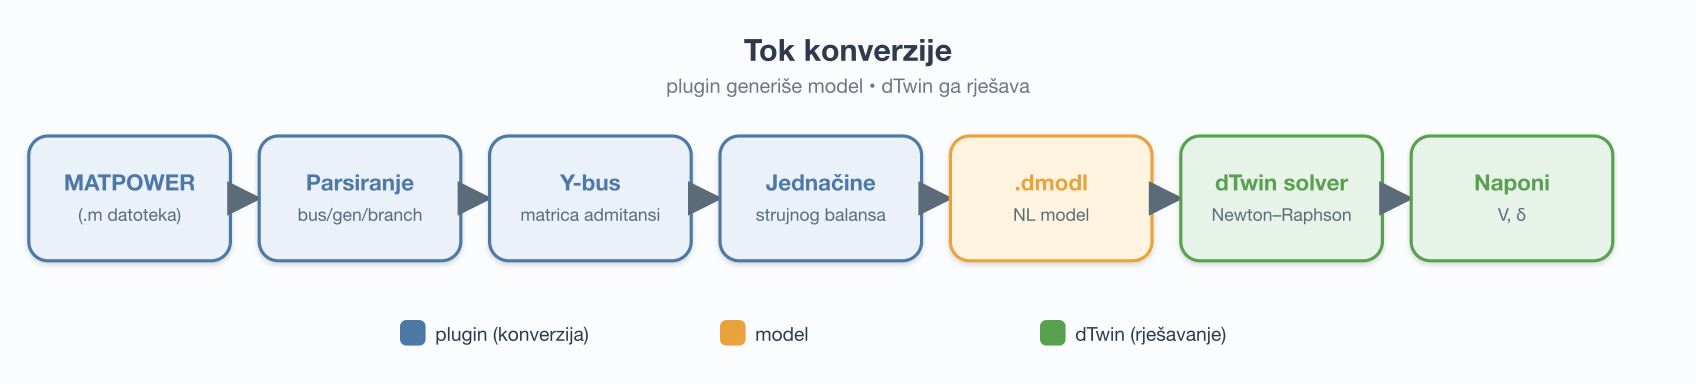
\includegraphics[width=0.96\linewidth]{02_tok_konverzije.png}

  \vspace{2mm}
  \small parsiranje \texttt{.m} $\rightarrow$ p.u.\ normalizacija $\rightarrow$
  Y-bus $\rightarrow$ ispis jednačina u \texttt{.dmodl} $\rightarrow$
  dTwin NL rješavač
\end{frame}

% ---- 6: implementacija --------------------------------------------------------
\begin{frame}{Implementacija (plugin)}
\begin{columns}[T]
\begin{column}{0.52\linewidth}
  \textbf{Struktura koda}
  \begin{itemize}
    \item \texttt{Converter.h} --- jezgra: parsiranje, Y-bus,
          generisanje \texttt{.dmodl};
    \item \texttt{CBPlugin.cpp} --- \texttt{sc::IPlugin} +
          \texttt{getPluginInterface()};
    \item \texttt{ViewConv.h} --- GUI: izbor datoteka, dugme,
          progres-bar, status;
    \item učitavanje: \textbf{Model $\rightarrow$ Import}, tip NL.
  \end{itemize}
\end{column}
\begin{column}{0.44\linewidth}
  \begin{block}{Višenitnost}
    \begin{itemize}
      \item konverzija u \texttt{std::thread} radniku
            (GUI ne blokira);
      \item progres na glavnoj niti:\\
            \texttt{asyncExecInMainThread}.
    \end{itemize}
  \end{block}
  \begin{block}{Izlaz}
    \begin{itemize}
      \item \texttt{.dmodl} preko \texttt{std::ofstream};
      \item + izlazna arhiva preko \texttt{put()}.
    \end{itemize}
  \end{block}
\end{column}
\end{columns}
\end{frame}

% ---- 7: rezultat — shema ------------------------------------------------------
\begin{frame}{Rezultat --- case9 (WSCC 9 čvorova)}
  \centering
  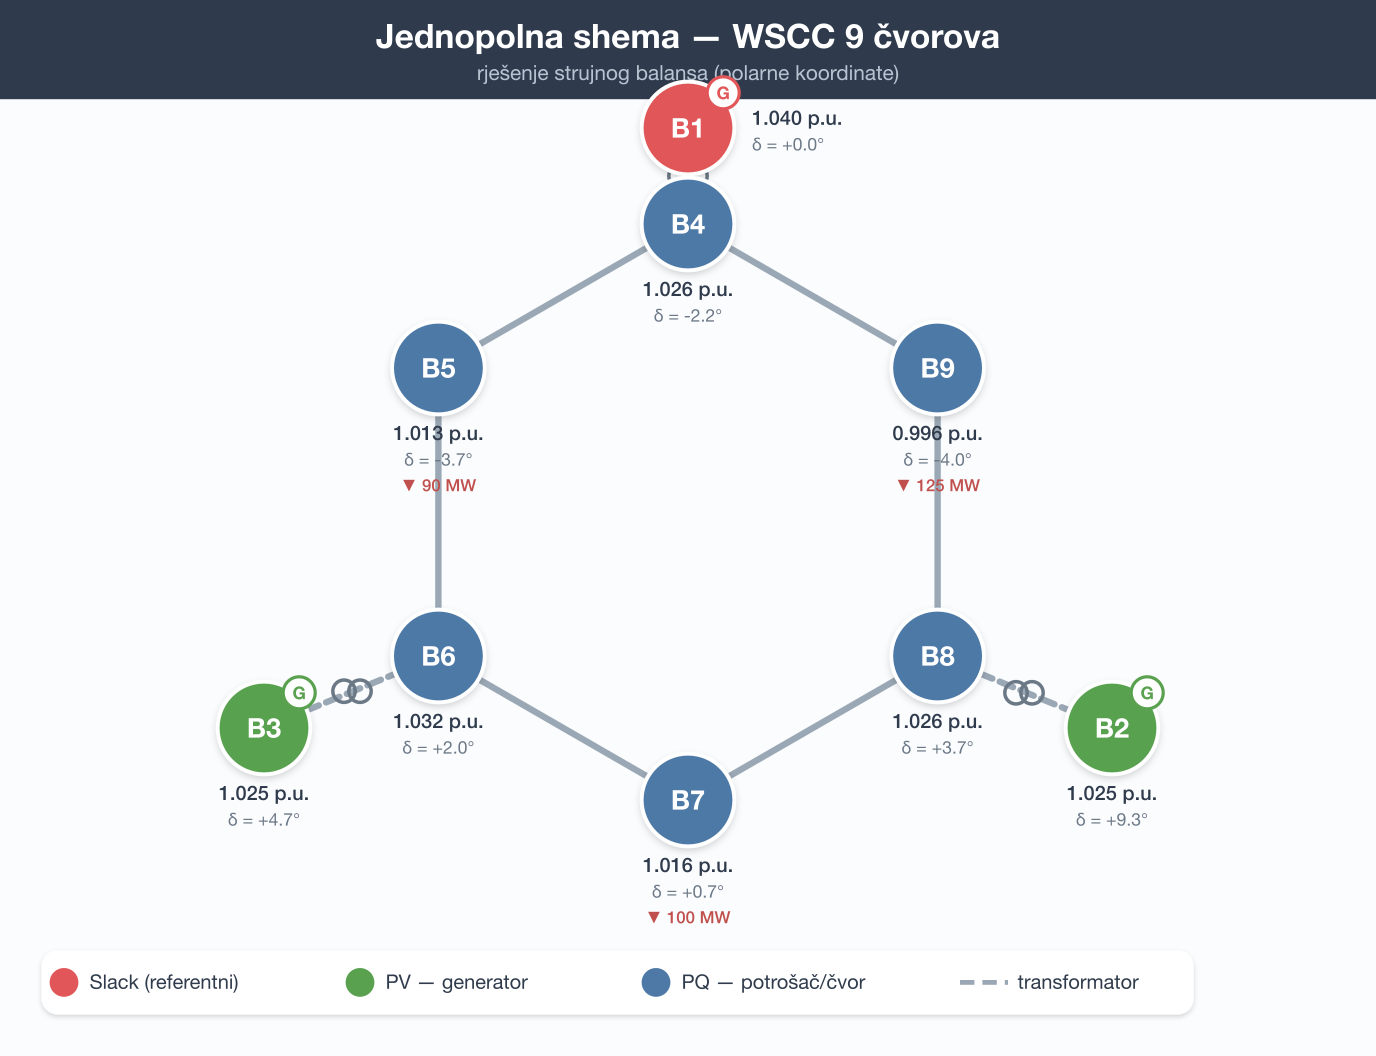
\includegraphics[height=0.82\textheight]{01_jednopolna_case9.png}
\end{frame}

% ---- 8: validacija ------------------------------------------------------------
\begin{frame}{Validacija (3 nezavisne provjere)}
\begin{columns}[T]
\begin{column}{0.52\linewidth}
  \begin{enumerate}
    \item Y-bus $=$ referentni \texttt{case9.dmodl}
          (\alert{10+ cifara});
    \item reziduali u tačnom rješenju:
          \alert{$2.4\cdot10^{-13}$}\\
          (nezavisna Python/numpy provjera);
    \item dTwin \texttt{modSolver} riješio generisani model:
          status \alert{\textbf{OK}}.
  \end{enumerate}
  \vspace{1mm}
  \begin{itemize}
    \item Newton--Raphson: konvergencija u \alert{4 iteracije}
          iz ravnog starta;
    \item PV čvorovi tačno izračunali $Q_g$.
  \end{itemize}
\end{column}
\begin{column}{0.44\linewidth}
  \centering
  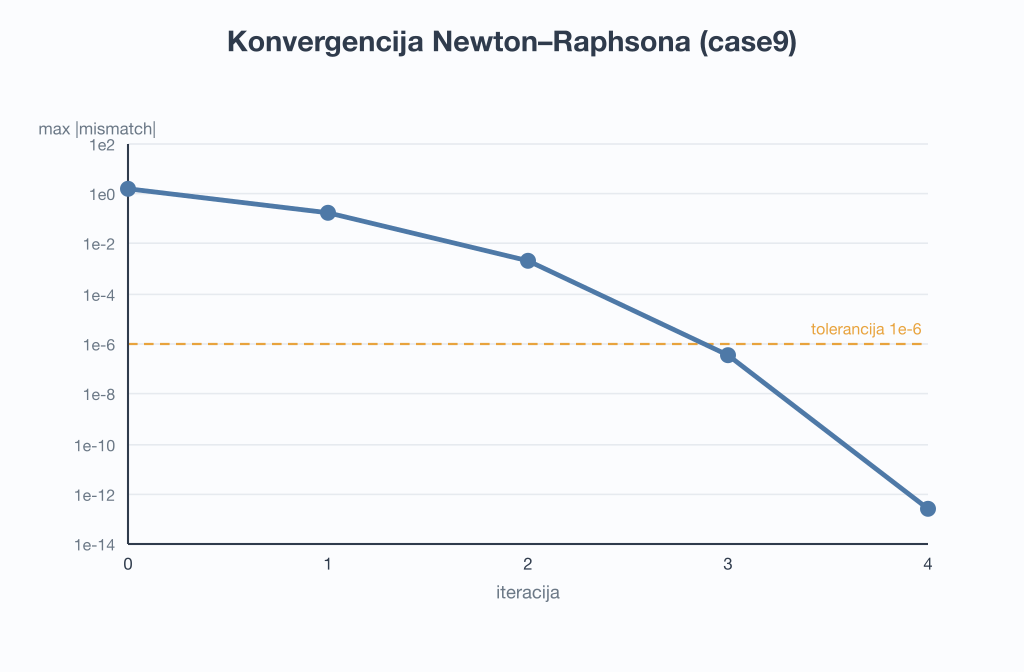
\includegraphics[width=\linewidth]{04_konvergencija.png}

  \scriptsize kvadratno opadanje reziduala po iteracijama
\end{column}
\end{columns}
\end{frame}

% ---- 9: tabela poređenja ------------------------------------------------------
\begin{frame}{Rezultat vs.\ referenca (case9)}
\begin{columns}[T]
\begin{column}{0.56\linewidth}
  \centering\small
  \begin{tabular}{c|cc|cc}
  \toprule
  Čvor & $V$ (dTwin) & $V$ (ref.) & $\delta\,[^\circ]$ (dTwin) & $\delta\,[^\circ]$ (ref.) \\
  \midrule
  1 & 1.0400 & 1.0400 & 0.00 & 0.00 \\
  2 & 1.0250 & 1.0250 & 9.28 & 9.28 \\
  3 & 1.0250 & 1.0250 & 4.66 & 4.66 \\
  4 & 1.0258 & 1.0258 & $-2.22$ & $-2.22$ \\
  5 & 1.0127 & 1.0127 & $-3.69$ & $-3.69$ \\
  6 & 1.0324 & 1.0324 & 1.97 & 1.97 \\
  7 & 1.0159 & 1.0159 & 0.73 & 0.73 \\
  8 & 1.0258 & 1.0258 & 3.72 & 3.72 \\
  9 & 0.9956 & 0.9956 & $-3.99$ & $-3.99$ \\
  \bottomrule
  \end{tabular}

  \vspace{2mm}
  \alert{\textbf{Poklapanje na 4+ decimale.}}
\end{column}
\begin{column}{0.40\linewidth}
  \centering
  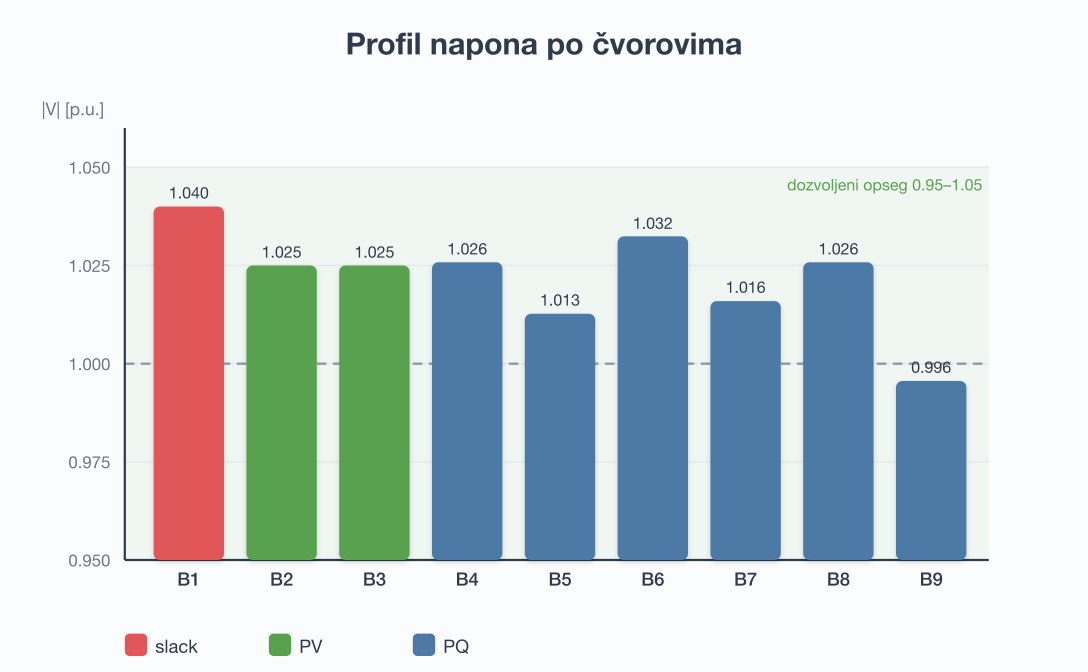
\includegraphics[width=\linewidth]{03_profil_napona.png}

  \vspace{1mm}
  \scriptsize Lijevo: dTwin \texttt{modSolver} nad generisanim modelom.\\
  Referenca: MATPOWER \texttt{case9} / provjereni Newton--Raphson.
\end{column}
\end{columns}
\end{frame}

% ---- 10: zaključak ------------------------------------------------------------
\begin{frame}{Zaključak}
  \begin{itemize}
    \item Konvertor strujnog balansa (polarne koordinate) ---
          \textbf{implementiran i validiran}.
    \item Trostruka validacija: Y-bus na 10+ cifara, reziduali
          $\sim 10^{-13}$, dTwin solver \textbf{OK} u 4 iteracije.
    \item Ispunjeni svi zahtjevi teme: C++, threading, real-time progres,
          GUI, plugin/\texttt{dll}.
    \item Sve matrice preko natID-a: Y-bus u \texttt{dense::CmplxMatrix}
          (potreban natID SDK \textbf{v4.2.0+}).
    \item Pravci proširenja: rijetka struktura za velike mreže,
          $Q_g$ limiti (PV$\rightarrow$PQ), veći MATPOWER slučajevi.
  \end{itemize}
  \vspace{3mm}
  \centering\large\textbf{Hvala na pažnji!}
\end{frame}

\end{document}
